
    
   Out of the two tasks of the competition, we implemented two different models (SVM and CRF) for the Drug Name Recognition task (task 9.1) and one model (SVM) for the Drug-Drug Interaction task (task 9.2). This section introduces the general approach followed for each of the models implemented. A general schema is shown in figure \ref{architecture}. The different ideas for features and model configuration have been extracted from different papers $\cite{liu_tang_chen_wang_fan_2015,kim_liu_yeganova_wilbur_2015,ratinov_roth_2009,liu_tang_chen_wang_2015}$.\\
   
\begin{figure}[H]
\centering
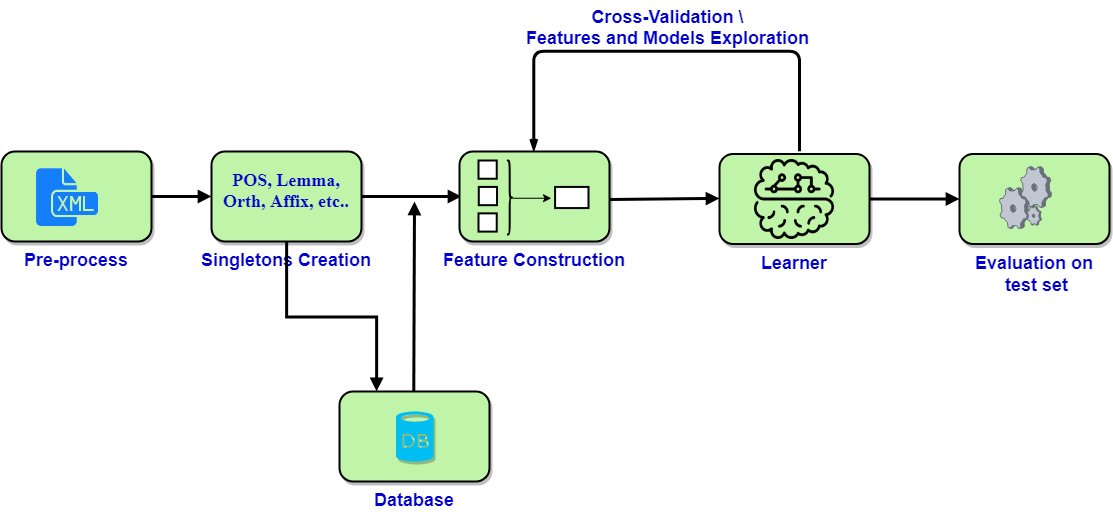
\includegraphics[scale=0.3]{ProcessCV.png}\caption{architecture}\label{architecture}
\end{figure}

   Our implementation, based on Python 3, starts with the parsing of the xml files that contain training and test samples of medical texts with two or more drugs mentioned in it. This first component basically traverses the folder that contains a set of xml files and creates a Python dictionary out of the information in it.\\
   The next software component, is in charge of extracting all the features that our learner model will use to train or to predict. This includes the most basic ones, already present in the xml file, like the word or sentence, or derived features like the BIO tag, the type of interaction for each drug pair , the POS-tag, lemma and orthographic features, all extracted using Freeling from the Python API. Finally, for more complex features, like Word2vec coordinates, dictionary lookup or dependency tree trigram frequencies, this component will write intermediate and final results to a file on disk.\\
   The next module in the chain will be in charge of selecting from the generated features (from memory or disk), the final feature vector that will be feed to the model for training or prediction  according to a configuration file that orchestrated the whole process.\\
   Finally, a learning model will be created and will use the features from the training data set to be trained and the features from the test data set to perform the predictions and evaluate its performance. We used scikit-learn and sklearn-crfsuite for the implementation of the learners.\\
   Due to our constrained time and resources, we performed feature selection and model selection by exploring different configurations of features and models in the two training and testing datasets. Our preferred approach would have been to preform model selection using crossvalidation before evaluating the selected model in the test set. Feature selection could also be done based on an analysis of the data and features, like frequency of appearance of each feature or entropy analysis.\\
   
   The models are trained from the training set of both Drugbank and Medline all mixed, but tested on each test set separately, in order to be able to use the official evaluation java code for the task 9.1 and 9.2 of SemEval'13. \\
   
The different experiments include exploring the results of training the svm model with different sets of features and window sizes, as well as with different model parameters. All the experiments are orchestrated by configuration files using the YAML format, where keys and values define the training and test set, the type of model, the features and window size as well as saving the results of the evaluation of the model.

  Further sections will explain the specific implementation for each trainer model and task.
    
